The gripper is selected according to payload, gripping force and opening width. The
opening width is the dominant selection criterion here, as the gripper must be able to grip both the thin
sheets with thicknesses of around 1 to 3 mm and the handle on the drawers with a width of 15 mm. An
electric gripper was considered, as the power supply could have been provided via the cable
already integrated in the robot. Due to the higher costs, the double height and the weight, a pneumatic
gripper was chosen. 


\begin{table}[h!]
    \centering
    \small
    \renewcommand{\arraystretch}{1.2} % Adjusts row height
    \begin{tabular}{l@{\hskip 2cm}l}
        \textbf{Description} & \textbf{Value} \\ \hline
        Closing Force & 550.0 N \\
        Stroke per jaw &  8.0 mm\\
        Min. operating pressure & 2.0 bar\\
        Max. operating pressure & 8.0 bar \\
        Opening force & 610.0 N\\
        Weight & 0.51 kg\\
        Opening time & 0.035 s\\
        Closing time & 0.035 s \\
        Repeat accuracy & 0.01 mm\\
        Size ($L \times W \times H$) & $96.0 \times 42.0 \times 49.0$ mm\\
        Min. Ambient temperature & 5.0\textdegree \\
        Max. Ambient temperature & 90.0\textdegree\\
        \hline
    \end{tabular}
    \caption{Schunk gripper technical details (Source: \cite{schunk-gripper})}
    \label{visor-technical-data}
\end{table}


\begin{figure}[h]
    \centering
    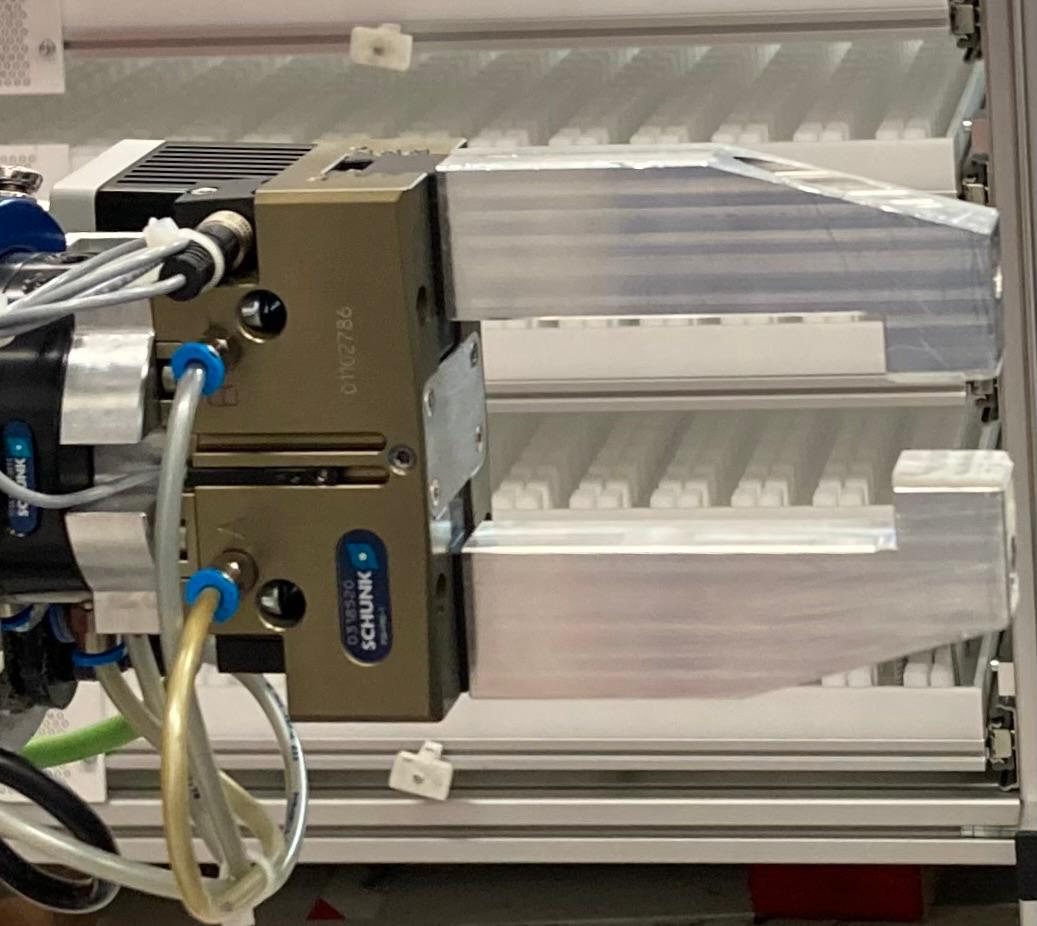
\includegraphics[width=0.5\textwidth]{figures/gripper.jpeg}
    \caption{Schunk gripper}
    \label{fig:schunk-gripper}
\end{figure}


A universal schunk gripper PGN-plus-P 80-1 is chosen which is a 
2-finger parallel pneumatic gripper with permanent lubrication, high gripping force, and high maximum moments due to the use of a multi-tooth guidance. \cite{schunk-gripper}
It is also possible to know if the gripper is open or closed because of a sensor inside the housing of gripper. This value of sensor is sent to the PLC to detect if the gripper is closed.


\subsubsection{Robotic Gripper}
\label{subsubsec:robotic-gripper}
The robotic gripper is mounted on the KR1410. This gripper is used for grasping the sheet metal parts, perfrom bending operation and opening or closing the drawers of shelf.

\subsubsection{Unloading Station Gripper}
\label{subsubsec:unloading-gripper}
The pneumatic parallel gripper is mounted on the pneumatic swivel unit which can turn 180\textdegree. This allows the transfer the 
sheet metal part from unloading station to the robotic gripper.